\chapter{DESIGN}
\section{Conceptual Design}
\subsection{Entity Types}
	\begin{longtable}{| p{3.5cm} | p{4.0cm} | l | p{4.5cm} |}
		\hline
		Entity Name & Description & Aliases & Occurence \\
		\hline \hline
		User & Berisi tentang informasi dan status session pengguna pada website & - & Setiap user akan memiliki tiga tipe pengguna dengan tujuannya masing-masing, yaitu user, supplier, dan designer \\ \hline
		UserInfo & Berisi tentang informasi pribadi pengguna website & - & Setiap user dapat melakukan pergantian informasi sesukanya \\
		UserPhoto & Akan menjadi data untuk penyimpanan dan pengaksesan foto profil pengguna & - & Setiap user dapat melihat sekaligus melakukan pergantian foto profil \\ \hline
		UserFeedback & Menjadi wadah bagi user untuk mengirim saran atau masukan kepada developer & - & Setiap user dapat mengirim saran dan pesan lebih dari satu kali \\ \hline
		ChatSystem & Sistem chatting antara pengguna kepada supplier atau pengguna kepada designer & - & User dapat dihadapkan kepada sistem chatting saat akan/ingin melakukan pembelian desain \\ \hline
		DesignCategories & Pilihan kategori atau peminatan sebuah desain & - & Setiap kategori telah ditetapkan secara spesifik dan mendetail \\ \hline
		DesignSubCategories & Pilihan sub-kategori atau jenis desain yang dibuat berdasarkan kategori yang ada & - & Setiap sub-kategori sudah ditetapkan mengikat pada kategori/peminatan desain yang telah ada \\ \hline
		DesignTheme & Pilihan tema sebuah desain & - & Tema akan ditempatkan pada masukan user. \\ \hline
		DesignHeader & Menjadi ikatan relasi antara kategori, sub-kategori, tema, dan supplier/designer. Entitas ini berfungsi sebagai identifikasi utama dari sebuah desain dan juga status penjualan desain & - & Ikatan - ikatan relasi yang ada akan ditetapkan oleh supplier/designer \\ \hline
		DesignLikeCount & Berfungsi menampung like dan dislike masukan dari pengguna website & - & Pemilihan like dan dislike akan ditentukan oleh pengguna \\ \hline
		UserInventory & Berisi desain - desain yang telah dibeli oleh pengguna dan dapat diakses kembali. & - & Entitas ini akan muncul saat pengguna telah membeli dan melakukan transaksi desain \\ \hline
		DesignTransaction Header & Berisi status dan identifikasi transaksi antara pengguna dengan desain yang akan atau telah dibeli & - & Transaksi akan muncul jika pengguna akan membeli desain yang diinginkan \\ \hline
		DesignTransaction Details & Berisi tanggal - tanggal dan informasi penting sebuah transaksi & - & Detail transaksi akan muncul seiring transaksi diadakan \\ \hline
		DesignDetails & Berisi informasi utama tentang desain yang dijual & - & Informasi ini akan ditetapkan oleh supplier dan akan muncul seiring relasi - relasi desain diadakan \\ \hline
		DesignPhotos & Berisi pratinjau foto - foto desain yang dijual & - & Foto - foto yang diperlukan akan diupload oleh supplier/designer \\ \hline
		DesignSpesification & Berisi spesifikasi mendetail tentang desain yang dijual  & - & Spesifikasi - spesifikasi ini dapat diisi oleh pengguna \\ \hline
		DesignFile & Berisi file desain secara teknis dan runtut & - & File dapat diakses oleh pengguna jika telah membeli dan membayar transaksi jual beli desain \\ \hline
		ExpoEvent & Berisi status dan relasi penting yang berkaitan dengan penyelenggaraan event expo & - & Jadwal dan status expo akan ditetapkan oleh supplier/designer sebagai penyelenggara \\ \hline
		ExpoTransaction Header & Berisi status utama transaksi tiket untuk mengikuti expo & - & Transaksi akan dimulai saat pengguna melakukan pembelian tiket expo \\ \hline
		UserExpo & Berisi expo - expo yang telah diikuti dan dibeli tiketnya oleh pengguna & - & Expo akan muncul pada entitas ini setelah tiket dibeli oleh pengguna \\ \hline
		ExpoTransaction Details & Berisi detail tanggal - tanggal dan status penting transaksi expo berjalan & - & Detail expo akan muncul seiring dengan status utama transaksi \\ \hline
		ExpoEventDetails & Berisi informasi penyelenggaraan expo secara mendetail & - & Informasi - informasi ini akan ditulis oleh supplier/designer \\ \hline
		ExpoEventPhoto & Berisi foto - foto dan pamflet yang berisi informasi penyelenggaraan expo & - & Supplier/Designer dapat melakukan proses upload pada entitas ini \\ \hline
		DesignerTransaction Header & Berisi informasi dan relasi utama transaksi antara pengguna user dan designer & - & Transaksi akan dimulai saat pengguna user akan melakukan persewaan designer \\ \hline
		DesignerTransaction Detail & Berisi informasi tanggal dan status penting berjalannya transaksi antara user dengan designer & - & Detail informasi akan muncul saat informasi transaksi utama muncul \\ \hline
		DesignerInfo & Berisi informasi  designer & - & Informasi akan ditetapkan oleh pengguna saat pengguna user melakukan pendaftaran menjadi desainer \\ \hline
		DesignerRating & Berfungsi untuk menampung masukkan rating atau penilaian oleh user lainnya & - & Pemilihan rating akan ditetapkan oleh user yang akan melakukan penilaian \\ \hline
		\caption{Entity Types}
	\end{longtable}

\subsection{Relationship Types}
	\begin{longtable}{| p{3.4cm} | l | l | l | p{3.4cm} |}
		\hline
		Entity Name & Multiplicity & Relationship & Multiplicity & Entity Name \\
		\hline
		User & 1 & Memiliki & 1 & DesignerInfo \\ \hline
		User & 0..1 & Berkaitan & 0..* & DesignerRating \\ \hline
		User & 0..* & Berkaitan & 0..* & ChatSystem \\ \hline
		User & 1 & Memiliki & 1 & UserInfo \\ \hline
		User & 1 & Memiliki & 1 & UserPhoto \\ \hline
		User & 0..* & Berkaitan & 1..* & UserFeedback \\ \hline
		User & 0..* & Berkaitan & 1..* & DesignTransaction Header \\ \hline
		User & 0..* & Berkaitan & 1..* & DesignLikeCount \\ \hline
		User & 0..* & Berkaitan & 1..* & UserExpo \\ \hline
		User & 0..* & Berkaitan & 1..* & DesignTransaction Header \\ \hline
		User & 0..* & Memiliki & 1..* & UserInventory \\ \hline
		User & 0..* & Berkaitan & 1..* & DesignHeader \\ \hline
		User & 0..* & Berkaitan & 1..* & ExpoTransaction Header \\ \hline
		User & 0..* & Berkaitan & 1..* & ExpoEvent \\ \hline
		DesignTransaction Header & 1 & Memiliki & 1 & DesignerTransaction Details \\ \hline
		DesignTransaction Header & 1 & Memiliki & 1 & DesignTransaction Details \\ \hline
		DesignTransaction Header & 1 & Berkaitan & 1 & UserInventory \\ \hline
		DesignHeader & 1 & Berkaitan & 1 & DesignTransaction Header \\ \hline
		DesignHeader & 1 & Berkaitan & 1 & UserInventory \\ \hline
		DesignHeader & 1 & Memiliki & 1 & DesignDetails \\ \hline
		DesignHeader & 1 & Berkaitan & 0..* & DesignLikeCount \\ \hline
		ExpoTransaction Header & 1 & Memiliki & 1 & ExpoTransaction Details \\ \hline
		ExpoEvent & 1 & Berkaitan & 1 & ExpoTransaction Details \\ \hline
		ExpoEvent & 1 & Berkaitan & 1..* & ExpoTransaction Header \\ \hline
		ExpoEvent & 1 & Memiliki & 1 & ExpoEventPhoto \\ \hline
		ExpoEvent & 1 & Memiliki & 1 & ExpoEventDetails \\ \hline
		DesignDetails & 1 & Memiliki & 1 & DesignPhotos \\ \hline
		DesignDetails & 1..* & Memiliki & 1 & DesignSpesification \\ \hline
		DesignDetails & 1 & Memiliki & 1 & DesignFile \\ \hline
		DesignCategories & 1 & Berkaitan & 1 & DesignHeader \\ \hline
		DesignCategories & 1..* & Berkaitan & 1 & DesignSubCategories \\ \hline
		DesignSubCategories & 1 & Berkaitan & 1 & Design Header \\ \hline
		DesignSubCategories & 1..* & Berkaitan & 1 & DesignTheme \\ \hline
		DesignTheme & 1 & Berkaitan & 1 & DesignHeader \\ \hline
		\caption{Relationship Types}
	\end{longtable}
\subsection{Attributes}
	\begin{longtable}{| p{2.2cm} | p{2.5cm} | p{3.4cm} | p{2.2cm} | l | p{1.3cm} |}
		\hline
		Entity Name & Attribute & Description & Data Type \& Length & Nulls & Multi valued \\
		\hline
		\noindent 
		User & 	UserId			& Identifikasi User			& Int(10)		& No & No \\
			 &	Email			& Email User				& Varchar(20)	& No & No \\
			 &	Password		& Password User				& Varchar(20)	& No & No \\
			 & 	LastActivity	& Terakhir kali user Aktif	& Datetime		& No & No \\
			 &	isOnline		& User sedang Online		& Boolean		& No & No \\
			 &	isSupplier		& User seorang supplier		& Boolean		& No & No \\
			 &	isDesigner		& User seorang designer		& Boolean		& No & No \\ \hline
			 
		UserInfo 	& UserId		& Identifikasi User		& Int(10)		& No  & No \\
					& Name			& Nama User				& Varchar(50)	& No  & No \\
					& Description	& Deskripsi supplier	& Text			& Yes & Yes \\
					& Company		& Perusahaan supplier	& Varchar(48)	& Yes & Yes \\
					& Location		& Lokasi Supplier		& Varchar(48)	& Yes & Yes \\
					& Website		& Website Supplier		& Varchar(48)	& Yes & Yes \\
					& PhoneNumber	& Nomor Telp Supplier	& Varchar(16)	& Yes & Yes \\ \hline
					
		UserPhoto	& PhotoId	& Identifikasi Foto	& Int(10)		& No & No \\
					& UserId	& Identifikasi User	& Int(10)		& No & No \\
					& PhotoName	& Nama Foto			& Varchar(48)	& No & No \\ \hline
					
		UserFeed-back	& FeedbackId		& Identifikasi		& Int(10) 	& No & No \\
						& UserId			& Identifikasi User	& Int(10) 	& No & No \\
						& Feedback-Message	& Isi Masukkan User	& Text		& No & Yes \\ \hline
						
		ChatSystem	& ChatSystemId	& Identifikasi Chat		& Int(10)		& No & No \\
					& toUserId		& Identifikasi tujuan	& Int(10)		& No & No \\
					& fromUserId	& Identifikasi asal		& Int(10)		& No & No \\
					& Message		& Isi Pesan				& Varchar(100)	& No & Yes \\
					& Timestamp		& Waktu Pengiriman		& Datetime		& No & No \\
					& StatusMessage	& Konfirmasi Terkirim	& Varchar(15)	& No & No \\ \hline
					
		Design-Categories	& CategoryId	& Identifikasi kategori	& Int(10)		& No  & No \\
							& CategoryName	& Nama Kategori			& Varchar(20)	& No  & No \\
							& CategoryDesc	& Deskripsi kategori	& Text			& Yes & No \\ \hline
		
		DesignSub-Categories	& SubCategoryId		& Identifikasi subkategori	& Int(10)		& No  & No \\
							& CategoryId		& Identifikasi kategori		& Int(10)		& No  & No \\
							& SubCategory-Name	& Nama subkategori			& Varchar(64)	& No  & No \\
							& SubCategory-Desc	& Deskripsi subkategori		& Text			& Yes & No \\ \hline
							
		DesignTheme	& ThemeId		& Identifikasi tema			& Int(10)		& No & No \\
					& SubCategoryId	& Identifikasi subkategori	& Int(10)		& No & No \\
					& ThemeName		& Nama tema					& Varchar(20)	& No & No \\ \hline

		DesignHeader	& DesignId			& Identifikasi desain		& Int(10)	& No & No \\
						& CategoryId		& Identifikasi kategori		& Int(10)	& No & No \\
						& SubCategoryId		& Identifikasi subkategori	& Int(10)	& No & No \\
						& ThemeId			& Identifikasi tema			& Int(10)	& No & No \\
						& SupplierUserId	& Identifikasi supplier		& Int(10)	& No & No \\
						& isSold			& Konfirmasi supply			& Boolean	& No & No \\ \hline
		
		DesignLike-Count	& LikeCountId	& Identifikasi like		& Int(10)	& No & No \\
						& DesignId		& Identifikasi desain	& Int(10)	& No & No \\
						& UserId		& Identifikasi user		& Int(10)	& No & No \\
						& Likes			& Total like			& Int(10)	& No & No \\ \hline
		
		UserInventory	& InventoryId			& Identifikasi kepemilikan		& Int(10)	& No & No \\
						& UserId				& Identifikasi User				& Int(10)	& No & No \\
						& DesignId				& Identifikasi Desain			& Int(10)	& No & No \\
						& DesignTransac-tionId	& Identifikasi					& Int(10)	& No & No \\
						& DatePurchased			& transaksi tanggal pembelian	& Datetime	& No & No \\ \hline
						
		Design-Transaction-Header	& Design-TransactionId	& Identifikasi Transaksi	& Int(10)	& No & No \\
									& DesignId				& Identifikasi Desain		& Int(10)	& No & No \\
									& BuyerUserId			& Identifikasi User			& Int(10)	& No & No \\
									& IsSuccess				& Konfirmasi sukses			& Boolean	& No & No \\
									& IsExpired				& Konfirmasi kadaluarsa		& Boolean	& No & No \\
									& Transaction-Type		& Tipe Transaksi			& Enum		& No & No \\ \hline
									
		Design-Transaction-Details	& Design-TransactionId	& Identifikasi transaksi	& Int(10)	& No & No \\
									& Design-Transaction-Date & Tanggal transaksi			& Datetime	& No & No \\
									& ExpirationDate		& Tanggal Kadaluarsa		& Datetime	& No & No \\
									& DateCreated			& Tanggal Dibuat			& Datetime	& No & No \\ \hline
		
		Designdetails	& DesignId			& Identifikasi desain		& Int(10)		& No & No \\
						& DesignName		& Nama Desain				& Varchar(64)	& No & No \\
						& DesignDesc		& Deskripsi Desain			& Text			& No & No \\
						& DesignPrice		& Harga Desain				& Int(10)		& No & No \\
						& DesignDate-Created & Tanggal Perilisan Desain	& Datetime		& No & No \\ \hline
		
		DesignPhotos	& DesignPhotoId		& Identifikasi foto		& Int(10)		& No & No \\
						& DesignId			& Identifikasi desain	& Int(10)		& No & No \\
						& Design-PhotoName	& Nama foto				& varchar(64)	& No & No \\ \hline
						
		Design-Spesification	& SpesificationId	& Identifikasi spesifikasi	& Int(10)		& No & No \\
								& DesignId			& Identifikasi desain		& Int(10)		& No & No \\
								& Spesification-Name	& Nama Spesifikasi			& Varchar(32)	& No & No \\
								& Spesification-Desc	& Deskripsi Spesifikasi		& Varchar(32)	& No & No \\ \hline
		
		DesignFile	& DesignFileId		& Identifikasi File		& Int(10)		& No & No \\
					& DesignId			& Identifikasi desain	& Int(10)		& No & No \\ 
					& DesignFileName	& Nama file desain		& varchar(20)	& No & No \\
					& DesignFileType	& Tipe file desain		& varchar(20)	& No & No \\ \hline
		
		ExpoEvent	& ExpoEventId		& Identifikasi expo			& Int(10)	& No & No \\
					& OrganizerUserId	& Identifikasi pembuat expo	& Int(10)	& No & No \\
					& CategoryId		& Kategori Expo				& Int(10)	& No & No \\
					& DateHeld			& Tanggal dibuat			& Datetime	& No & No \\
					& IsOnline			& Tipe Expo					& Boolean	& No & No \\ \hline

		Expo-Transaction-Header	& Expo-TransactionId	& Identifikasi transaksi	& Int(10)		& No & No \\
								& ExpoEventId		& Identifikasi event		& Int(10)		& No & No \\
								& BuyerUserId		& Identifikasi pembeli		& Int(10)		& No & No \\
								& IsSuccess 		& Konfirmasi pembelian		& Boolean		& No & No \\
								& IsExpired			& Konfirmasi kadaluarsa		& Boolean		& No & No \\
								& Transaction-Type	& Jenis transaksi			& Varchar(32)	& No & No \\ \hline
		
		UserExpo	& UserId			& Identifikasi User			& Int(10)	& No & No \\
					& ExpoEventId		& Identifikasi expo			& Int(10)	& No & No \\
					& Expo-TransactionId	& Identifikasi transaksi	& Int(10)	& No & No \\
					& DatePurchased		& Tanggal Pembelian			& Datetime	& No & No \\ \hline
		
		Expo-Transaction-Details	& Expo-Transaction-Id		& Identifikasi transaksi	& Int(10)	& No & No \\
								& Expo-Transaction-Date	& Tanggal transaksi			& Datetime	& No & No \\
								& Expo-Expiration-Date	& Tanggal kadaluarsa tiket	& Datetime	& No & No \\
								& DateCreated			& Tanggal expo dibuat		& Datetime	& No & No \\ \hline
								
		Expo-Event-Details	& ExpoEventId		& Identifikasi event	& Int(10)		& No  & No \\
							& ExpoEventTitle	& Nama event			& Varchar(32)	& No  & No \\
							& ExpoEvent-Place	& Tempat Event			& Varchar(32)	& No  & Yes \\
							& ExpoEventLink		& Link Event			& Varchar(32)	& Yes & Yes \\
							& ExpoEventDesc		& Deskripsi Event		& Text			& No  & No \\
							& TicketQuota		& Kuota Event			& Int(10)		& No  & No \\
							& TicketPrice		& Harga Tiket			& Int(10)		& No  & No \\ \hline
							
		Designer-Transaction-Header	& Designer-TransactionId	& Identifikasi Transaksi	& Int(10)		& No & No \\
									& DesignerId			& Identifikasi Desainer		& Int(10)		& No & No \\
									& BuyerUserId			& Identifikasi Pembeli		& Int(10)		& No & No \\
									& IsSuccess				& Konfirmasi pembelian		& Boolean		& No & No \\
									& IsExpired				& Konfirmasi kadaluarsa		& Boolean		& No & No \\
									& Transaction-Type		& Jenis transaksi			& Varchar(32)	& No & No \\ \hline
									
		Designer-Transaction-Details	& Designer-TransactionId	& Identifikasi desainer	& Int(10)	& No & No \\
									& AssignedDate			& Tanggal mulai proyek	& Date		& No & No \\
									& DeadlineDate			& Tanggal akhir proyek	& Date		& No & No \\
									& Confirmed				& Konfirmasi proyek		& Boolean	& No & No \\ \hline
									
		DesignerInfo	& DesignerId	& Identifikasi Desainer		& Int(10)	& No & No \\
						& DesignerPrice	& Harga jasa desainer		& Int(10)	& No & No \\
						& Rating		& Total penilaian Desainer	& Int(10)	& No & No \\ \hline
						
		Designer-Rating	& RatingId		& Identifikasi Penilaian	& Int(10)	& No & No \\
						& DesignerId	& Identifikasi Desainer		& Int(10)	& No & No \\
						& UserId		& Identifikasi User			& Int(10)	& No & No \\
						& Rating		& Penilaian per user		& Int(10)	& No & No \\ \hline
		
		\caption{Attributes}
	\end{longtable}
\subsection{Attribute Domains}
List of attribute domain:
\begin{itemize}
	\item Atribut Rating pada tabel DesignerInfo adalah constraint yang bertipe integer dimana constraint ini berupa angka yang memiliki nilai minimal 1 serta maksimal 5.
	\item Atribut Rating pada tabel DesignerRating adalah constraint yang bertipe integer dimana constraint ini berupa angka yang memiliki nilai minimal 1 serta maksimal 5.
	\item Atribut PhoneNumber pada tabel UserInfo adalah constraint yang bertipe varchar dimana constraint ini memiliki panjang 13 karakter dimana karakter pertama dan kedua harus berupa angka “08” dan karakter selanjutnya berupa angka hingga mencapai 13 karakter.
	\item Atribut website pada tabel UserInfo adalah constraint yang bertipe varchar dimana constraint ini memiliki karakter berupa string yang diikuti oleh tanda titik (.), serta dilanjutkan oleh  karakter berupa string.
	\item Atribut email pada tabel User adalah constraint yang bertipe varchar dimana constraint ini memiliki karakter berupa string yang diikuti oleh tanda @, serta dilanjutkan oleh karakter berupa string lalu titik (.), dan dilanjutkan oleh karakter string.
	\item Atribut TicketQty pada tabel ExpoTransactionHeader adalah constraint yang bertipe integer dimana constraint ini berupa angka yang memiliki nilai maksimal 10.
	\item Atribut TicketQuota pada tabel ExpoEventDetails adalah constraint yang bertipe integer dimana constraint ini berupa angka yang memiliki nilai maksimal 10.
\end{itemize}

\subsection{Candidate Keys, Primary Key, and Alternate Keys}
	\begin{longtable}{| p{3cm} | p{3.2cm} | l | p{3.2cm} |}
		\hline
		Entity Name & Candidate Key & Primary Key & Alternate Key \\
		\hline
		User 						& UserId 				& UserId 				& x 					\\ \hline
		UserInfo 					& UserId 				& x 					& UserId 				\\ \hline
		UserPhoto 					& PhotoId 				& PhotoId 				& UserId 				\\
					 				& UserId				& 						&						\\ \hline
		UserFeedback				& FeedbackId			& FeedbackId			& UserId				\\
									& UserId				& 						&						\\ \hline
		ChatSystem					& ChatSystemId			& ChatSystemId			& toUserId				\\
									& toUserId				&						& fromUserId			\\
									& fromUserId			&						&						\\ \hline
		DesignCategories			& CategoryId			& CategoryId			& x						\\ \hline
		DesignSub-Categories			& SubCategoryId			& SubCategoryId			& CategoryId			\\
									& CategoryId			&						& 						\\ \hline
		DesignTheme					& ThemeId				& ThemeId				& SubCategoryId			\\
									& SubCategoryId			&						&						\\ \hline
		DesignHeader				& DesignId				& DesignId				& CategoryId			\\
									& CategoryId			&						& SubCategoryId			\\
									& SubCategoryId 		&						& ThemeId				\\
									& ThemeId				&						& SupplierUserId		\\
									& SupplierUserId		&						& 						\\ \hline
		DesignLikeCount				& LikeCountId			& LikeCountId			& DesignId				\\
									& DesignId				& 						& UserId				\\
									& UserId				& 						& 						\\ \hline
		UserInventory				& LikeCountId			& LikeCountId			& DesignId				\\
									& DesignId				& 						& UserId				\\
									& UserId				&						&						\\ \hline
		DesignTransaction-Header		& DesignTransactionId	& DesignTransactionId	& DesignId				\\
									& DesignId				&						& BuyerUserId			\\
									& BuyerUserId			&						&						\\ \hline
		DesignTransaction-Details	& Design-TransactionId	& x						& Design-TransactionId	\\ \hline
		DesignDetails				& DesignId				& x						& DesignId				\\ \hline
		DesignPhotos				& DesignPhotoId			& DesignPhotoId			& DesignId				\\
									& DesignId				&						& 						\\ \hline
		DesignSpesification			& SpesificationId		& SpesificationId		& DesignId				\\
									& DesignId				&						&						\\ \hline
		DesignFile					& DesignFileId			& DesignFileId			& DesignId				\\
									& DesignId				&						&						\\ \hline
		ExpoEvent					& ExpoEventId			& ExpoEventId			& OrganizerUserId		\\
									& OrganizerUserId		&						& CategoryId			\\
									& CategoryId			&						&						\\ \hline
		ExpoTransaction-Header		& Expo-TransactionId		& ExpoTransactionId		& ExpoEventId			\\
									& ExpoEventId			&						& BuyerUserId			\\
									& BuyerUserId			&						&						\\ \hline
		UserExpo					& UserId				& x						& UserId				\\
									& ExpoEventId			&						& ExpoEventId			\\
									& Expo-TransactionId		&						& Expo-TransactionId		\\ \hline
		ExpoTransaction-Details		& Expo-TransactionId		& x						& Expo-TransactionId		\\ \hline
		ExpoEvent-Details			& ExpoEventId			& x						& ExpoEventId			\\ \hline
		ExpoEvent-Photo				& PhotoId				& PhotoId				& ExpoEventId			\\
									& ExpoEventId			&						& 						\\ \hline
		Designer-Transaction-Header	& Designer-TransactionId	& DesignerTransactionId	& DesignerId			\\
									& DesignerId			& 						& BuyerUserId			\\
									& BuyerUserId			&						& 						\\ \hline
		Designer-Transaction-Details	& Designer-TransactionId	& x						& Designer-TransactionId	\\ \hline
		DesingerInfo				& DesignerId			& x						& DesignerId			\\ \hline
		DesignerRating				& RatingId				& RatingId				& DesignerId			\\
									& DesignerId			&						& UserId				\\
									& UserId				&						&						\\ \hline
									
		\caption{Candidate Keys, Primary Keys, dan Alternate Keys}
	\end{longtable}

\subsection{List of User Transaction}
\begin{center}
	\fbox{\begin{minipage}{17em}
			List of user transaction:
			\begin{enumerate}[A.]
				\item DesignTransactionHeader
				\item DesignTransactionDetails
				\item ExpoTransactionHeader
				\item ExpoTransactionDetails
				\item DesignerTransactionHeader
				\item DesignerTransactionDetail
			\end{enumerate}
	\end{minipage}}
\end{center}

\subsection{Entity Relationship Diagram}
\begin{figure}[h]
	\centering
	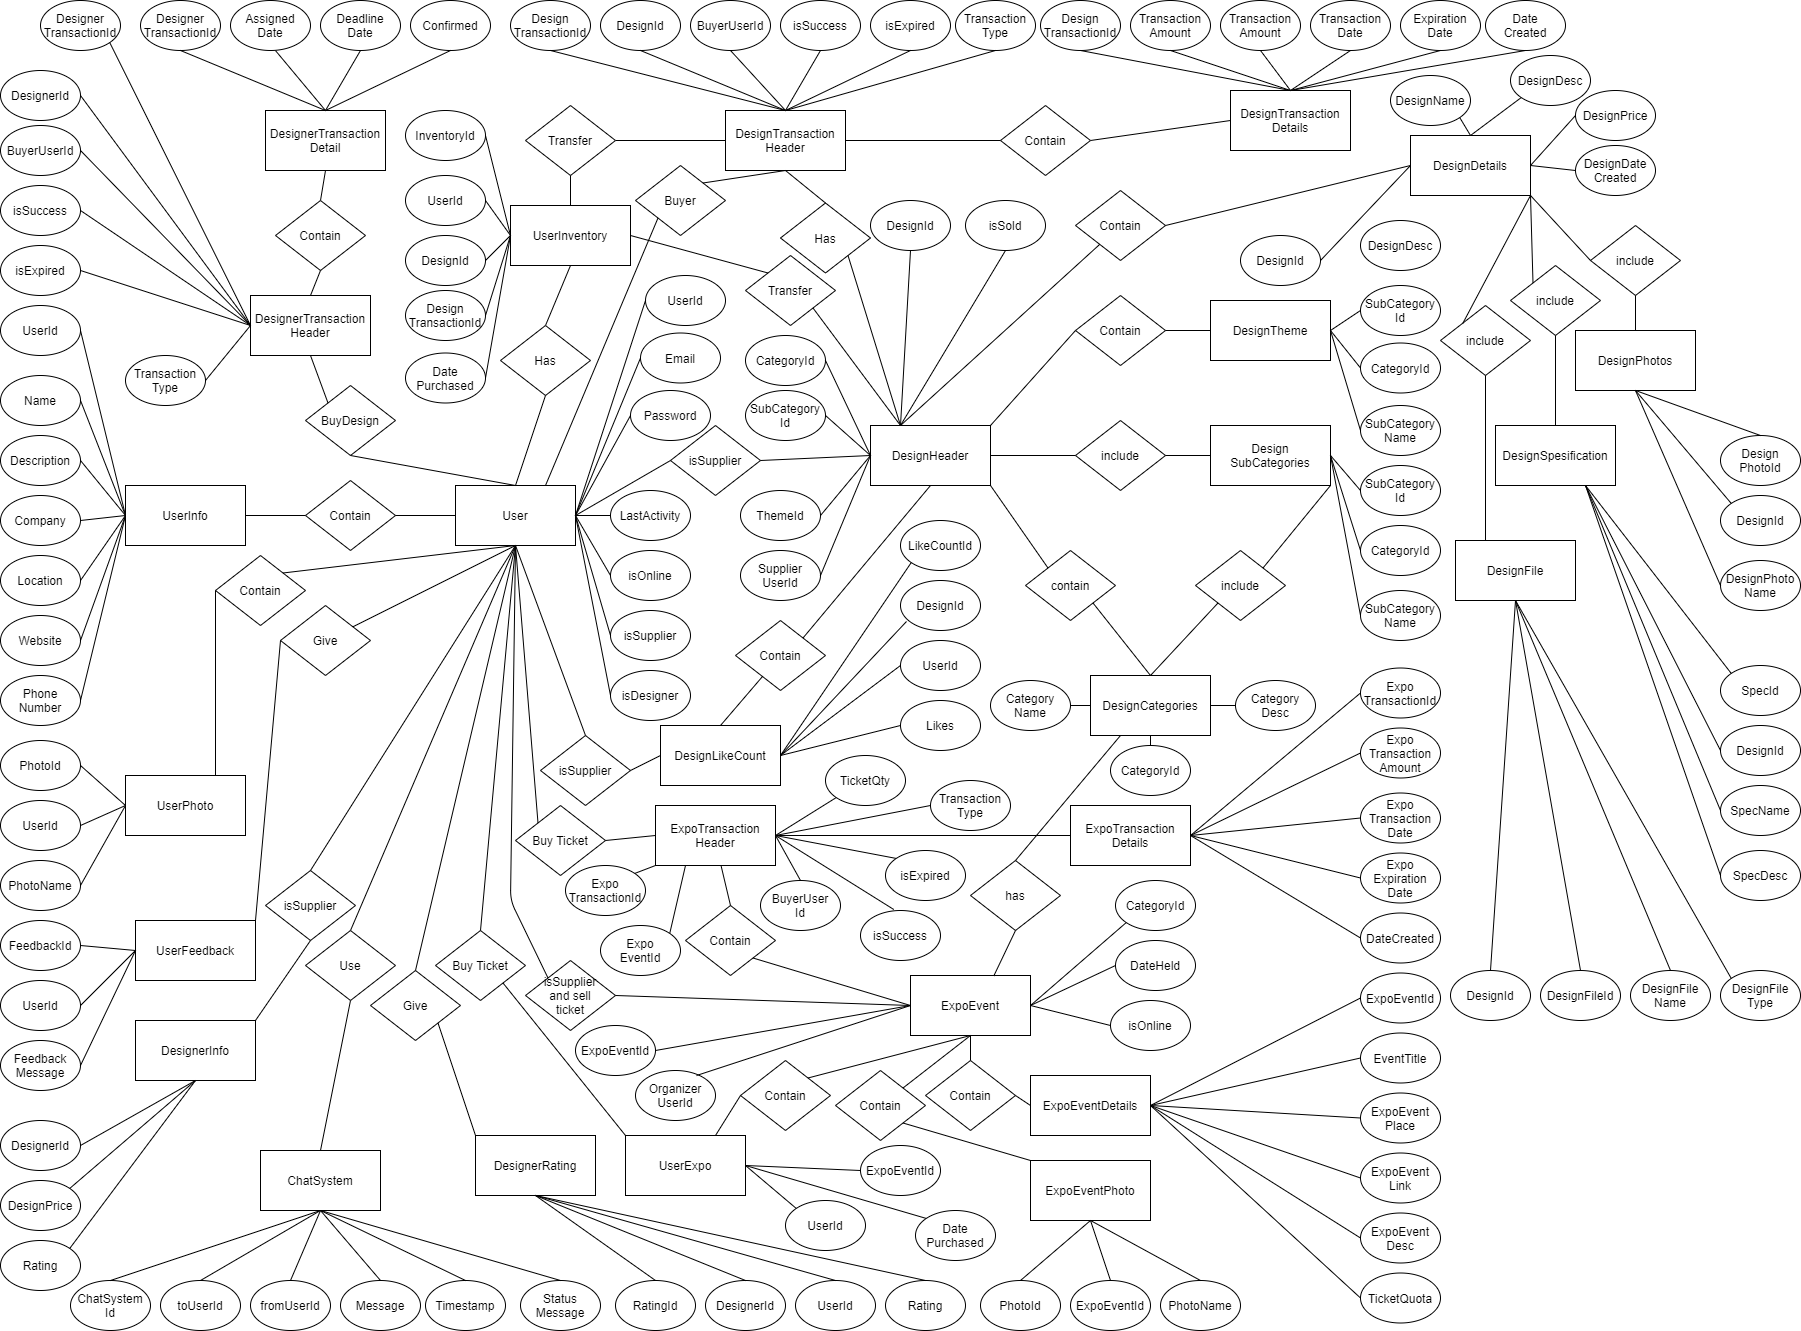
\includegraphics[width=\textwidth, height=\textheight, keepaspectratio]{erd}
	\caption{ERD Sistem Belidesain}
\end{figure}

\section{Logical Model (Class Diagram)}

\begin{figure}[H]
	\centering
	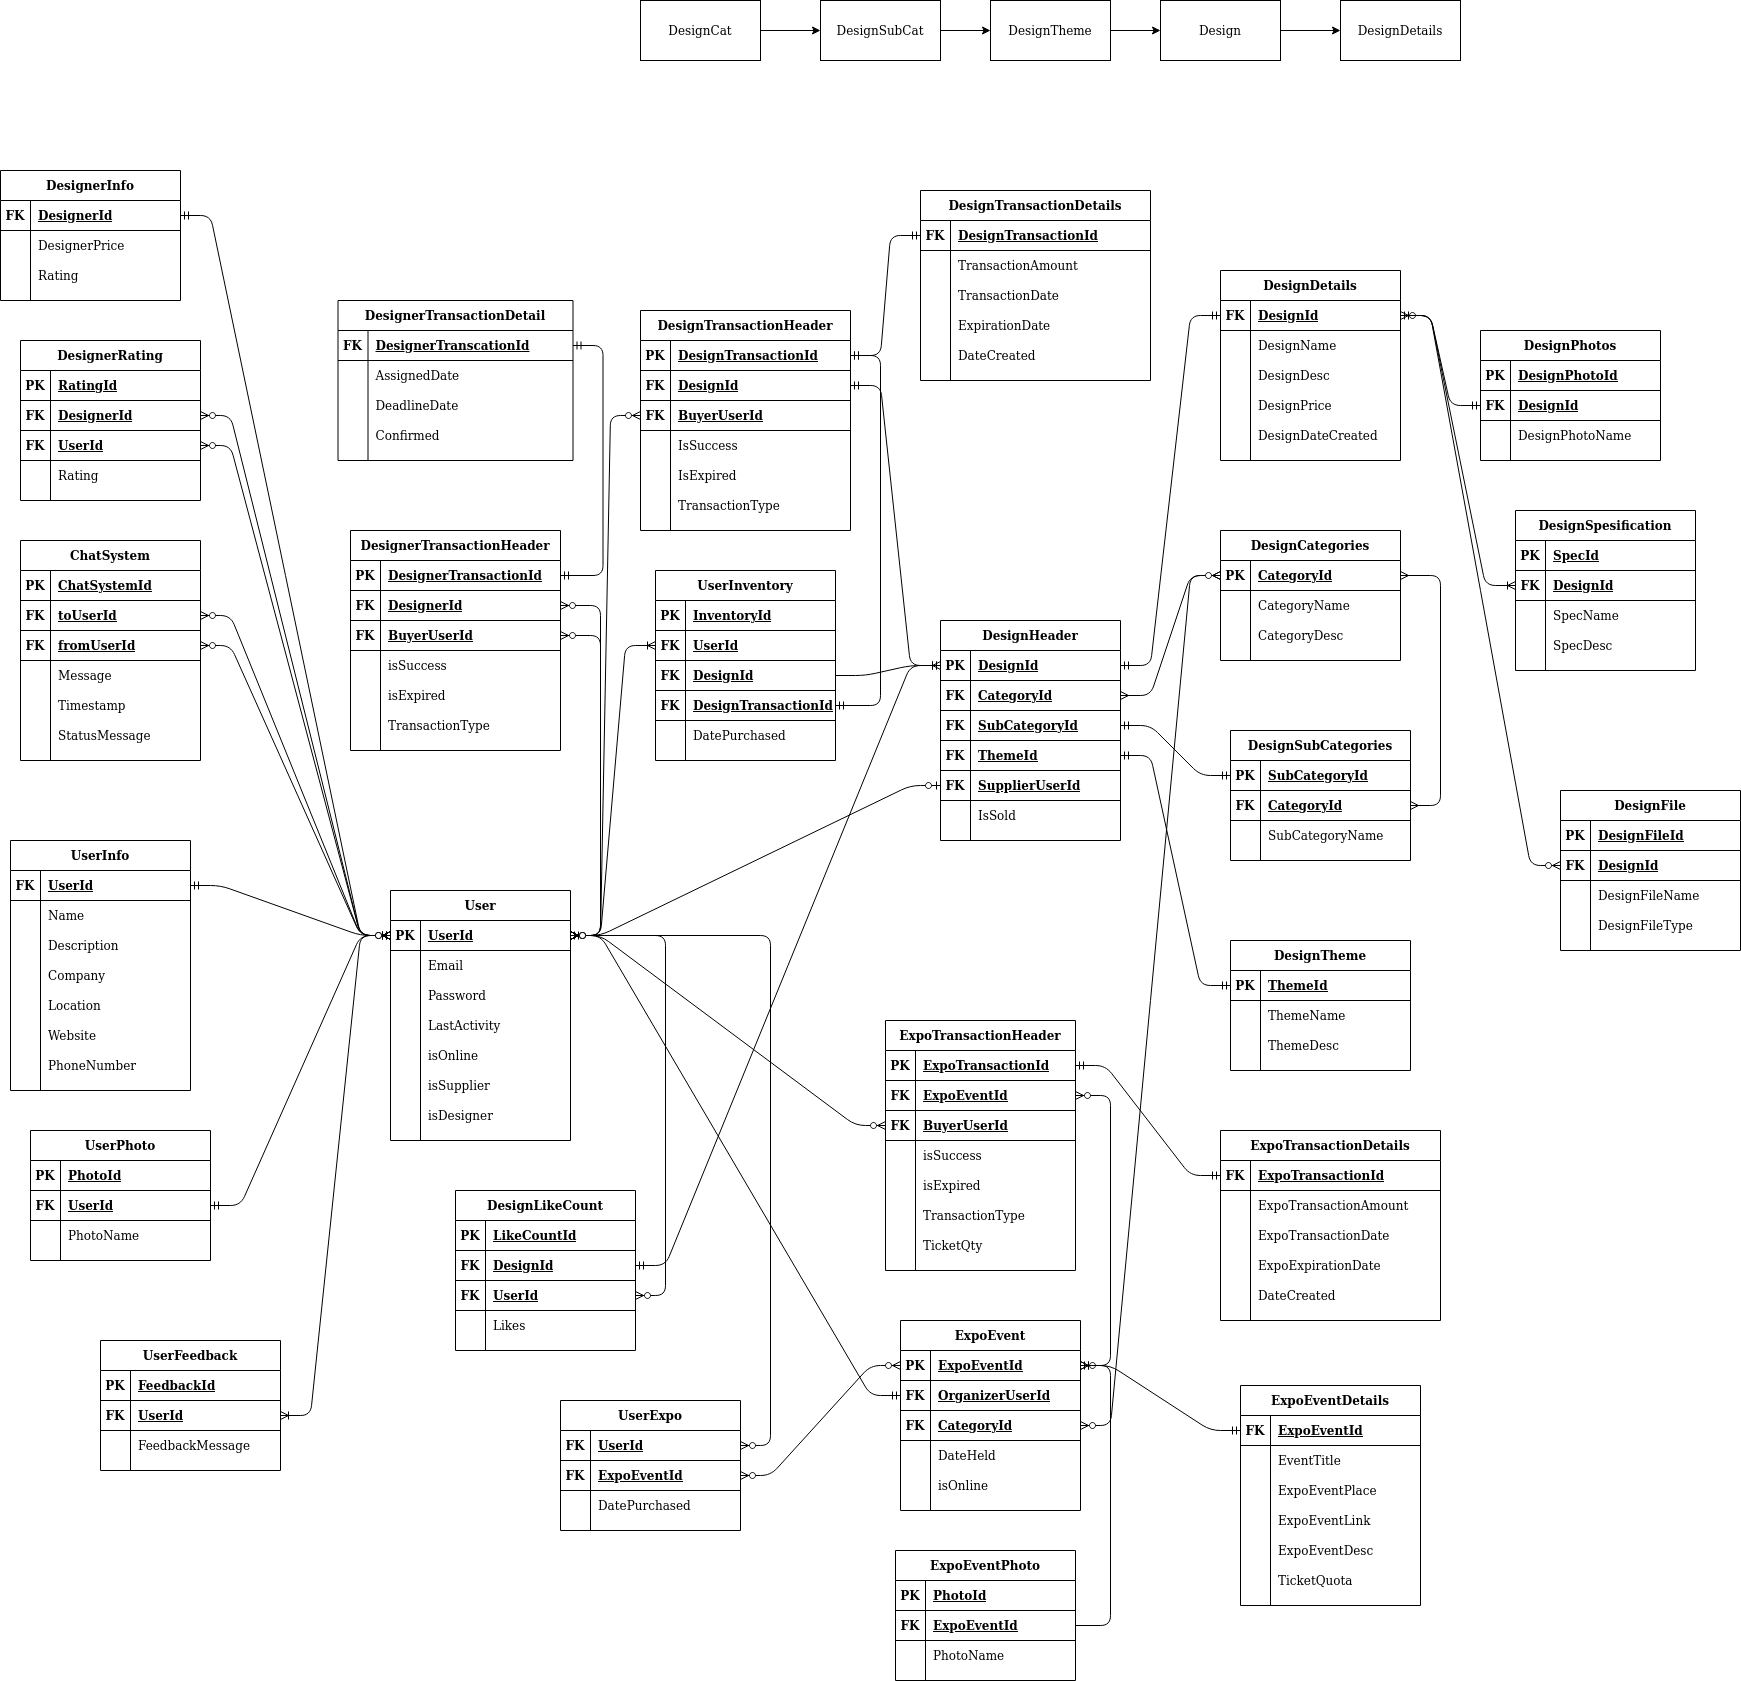
\includegraphics[width=\textwidth, height=\textheight, keepaspectratio]{classdiagram}
	\caption{Class Diagram Belidesain}
\end{figure}

\section{Physical Model}
\subsection{List of Index}
	\begin{longtable}{| p{3.0cm} | p{2.8cm} | p{3.0cm} | c | c |}
		\hline
		Entity Name 				& Index Name 			& Index 				& \multicolumn{2}{c|}{Type} \\ \cline{4-5}
									& 						&		 				& Clustered 	& Non-Clustered	\\ \hline
		User						& UserId				& UserId				& \checkmark 	& 				\\	\hline
		UserInfo					& 						&						&				& \checkmark	\\ \hline
		UserPhoto					& PhotoId				& PhotoId				& \checkmark	&				\\ \hline
		UserFeedback				& FeedbackId			& FeedbackId			& \checkmark	&				\\ \hline
		ChatSystem					& ChatSystemId			& ChatSystemId			& \checkmark	&				\\ \hline
		DesignCategories 			& CategoriesId			& CategoriesId			& \checkmark	&				\\ \hline
		DesignSub-Categories			& Sub-CategoriesId		& SubCategoriesId		& \checkmark	& 				\\ \hline
		DesignTheme					& ThemeId				& ThemeId				& \checkmark	&				\\ \hline
		DesignHeader				& DesignId				& DesignId				& \checkmark	&				\\ \hline
		DesignLikeCount				& LikeCountId			& LikeCountId			& \checkmark	& 				\\ \hline
		UserInventory				& InventoryId			& InventoryId			& \checkmark	&				\\ \hline
		DesignTransaction-Header		& Design-TransactionId	& Design-TransactionId	& \checkmark	& 				\\ \hline
		DesignTransaction-Details	& TransactionId			& TransactionId			& \checkmark	&				\\ \hline
		DesignDetails				&						&						&				& \checkmark	\\ \hline
		DesignPhotos				& DesignPhotoId			& DesignPhotoId			& \checkmark	&				\\ \hline
		DesignSpesification			& SpesificationId		& SpesificationId		& \checkmark	&				\\ \hline
		DesignFile					& DesignFileId			& DesignFileId			& \checkmark	&				\\ \hline
		ExpoEvent					& ExpoEventId			& ExpoEventId			& \checkmark	&				\\ \hline
		ExpoTransaction-Header		& ExpoTransaction-Id		& ExpoTransaction-Id		& \checkmark	&				\\ \hline
		UserExpo					& 						&						&				& \checkmark	\\ \hline
		ExpoTransaction-Header		& 						&						&				& \checkmark	\\ \hline
		ExpoEventDetails			&						&						&				& \checkmark	\\ \hline
		ExpoEventPhoto				&						&						&				& \checkmark	\\ \hline
		Designer-Transaction-Header	& Designer-TransactionId	& Designer-TransactionId	& \checkmark	&				\\ \hline
		Designer-Transaction-Details	&						&						&				& \checkmark	\\ \hline
		DesignerInfo				&						&						&				& \checkmark	\\ \hline
		DesignerRating				& RatingId				& RatingId				& \checkmark	&				\\ \hline
		\caption{List of Index}		
	\end{longtable}

\subsection{Analyze Transaction}
\definecolor{codegreen}{rgb}{0,0.6,0}
\definecolor{codegray}{rgb}{0.5,0.5,0.5}
\definecolor{codepurple}{rgb}{0.58,0,0.82}
\definecolor{backcolour}{rgb}{0.95,0.95,0.92}

\begin{table}[H]
	\centering
	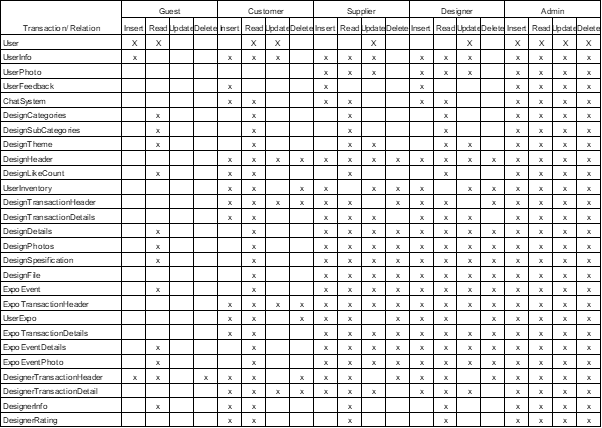
\includegraphics[width=\textwidth, height=\textheight, keepaspectratio]{analyzetransaction}
	\caption{Analyze Transaction}	
\end{table}
\subsection{User View, Procedure, and Function}
\subsubsection{Data Tabel}
\begin{table}[H]
	\centering
	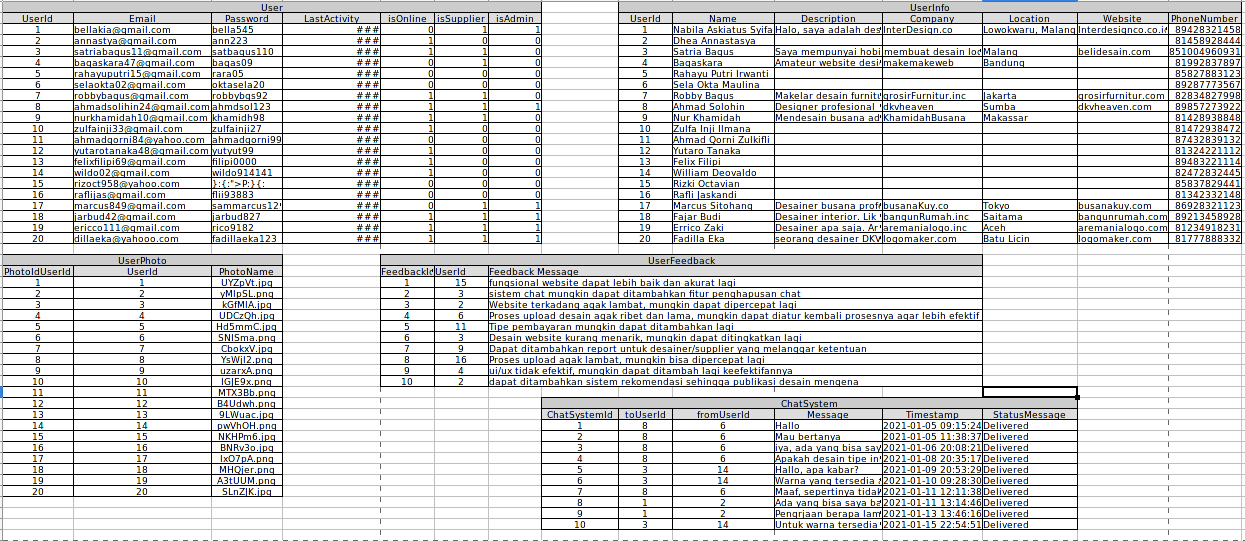
\includegraphics[width=\textwidth, height=\textheight, keepaspectratio]{insert1}
	\caption{Insert Table 1}
\end{table}
\begin{table}[H]
	\centering
	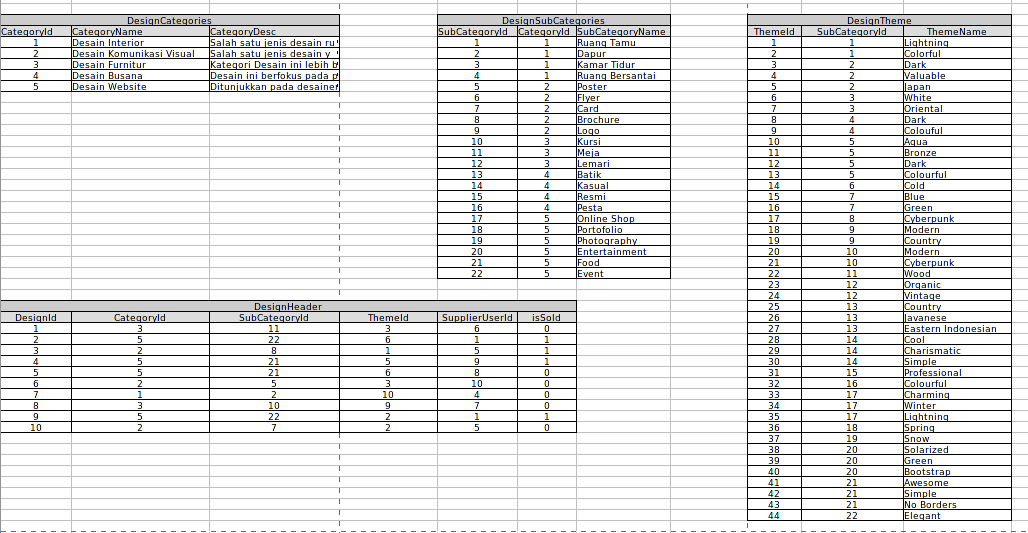
\includegraphics[width=\textwidth, height=\textheight, keepaspectratio]{insert2}
	\caption{Insert Table 2}
\end{table}
\begin{table}[H]
	\centering
	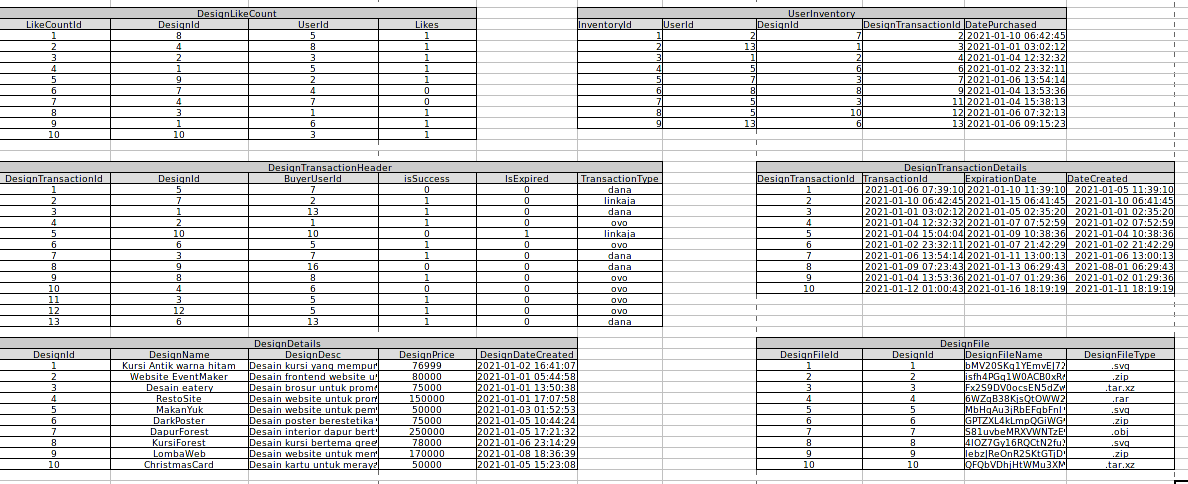
\includegraphics[width=\textwidth, height=\textheight, keepaspectratio]{insert3}
	\caption{Insert Table 3}
\end{table}
\begin{table}[H]
	\centering
	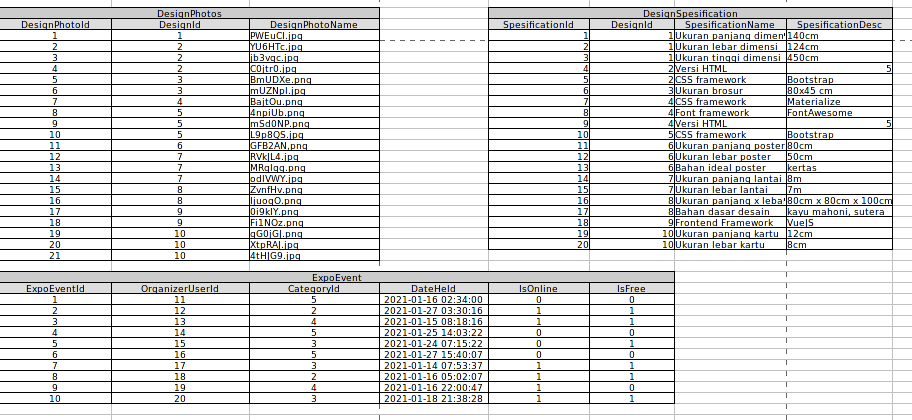
\includegraphics[width=\textwidth, height=\textheight, keepaspectratio]{insert4}
	\caption{Insert Table 4}
\end{table}
\begin{table}[H]
	\centering
	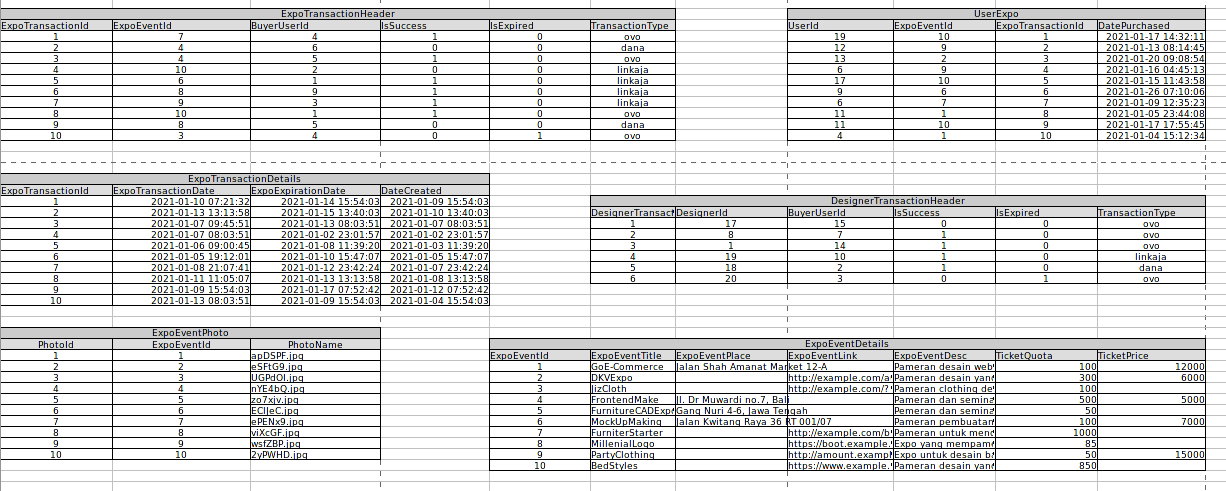
\includegraphics[width=\textwidth, height=\textheight, keepaspectratio]{insert5}
	\caption{Insert Table 5}
\end{table}
\begin{table}[H]
	\centering
	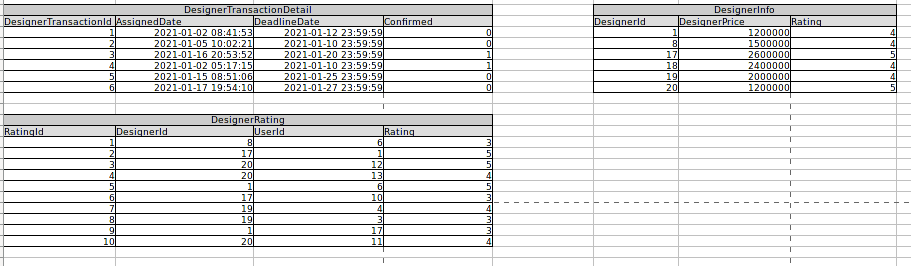
\includegraphics[width=\textwidth, height=\textheight, keepaspectratio]{insert6}
	\caption{Insert Table 6}
\end{table}
\subsubsection{User Views}
\begin{enumerate}
	\item 	Fungsi \textit{view} untuk melihat desainer dengan nilai \textit{rating} tertinggi sampai terendah \\
			Source Code :
			\begin{lstlisting}[
				language=SQL,
				backgroundcolor=\color{backcolour},   
				commentstyle=\color{codegreen},
				keywordstyle=\color{magenta},
				numberstyle=\tiny\color{codegray},
				stringstyle=\color{codepurple},
				basicstyle=\ttfamily\footnotesize,
				breakatwhitespace=false,         
				breaklines=true,                 
				captionpos=b,                    
				keepspaces=true,                 
				numbers=left,                    
				numbersep=5pt,                  
				showspaces=false,                
				showstringspaces=false,
				showtabs=false,                  
				tabsize=2]
	create view Designer_Rating_Tertinggi as
	select distinct B.Name, D.Rating
	from User A join UserInfo B
	on A.UserId = B.UserId
	join DesignerRating C
	on A.UserId = C.DesignerId
	join DesignerInfo D
	on D.DesignerId = C.DesignerId
	order by D.Rating desc;
		
	select * from Designer_Rating_Tertinggi;
	drop view Designer_Rating_Tertinggi;
			\end{lstlisting} 
		Hasil : 
		\\
		\begin{figure}[H]
			\centering
			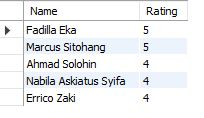
\includegraphics[width=0.4\textwidth]{view1}
			\caption{Hasil View 1}
		\end{figure}
	\item	Fungsi \textit{view} untuk melihat desain dengan harga tertinggi sampai terendah \\
			Source Code :
			\begin{lstlisting}[
				language=SQL,
				backgroundcolor=\color{backcolour},   
				commentstyle=\color{codegreen},
				keywordstyle=\color{magenta},
				numberstyle=\tiny\color{codegray},
				stringstyle=\color{codepurple},
				basicstyle=\ttfamily\footnotesize,
				breakatwhitespace=false,         
				breaklines=true,                 
				captionpos=b,                    
				keepspaces=true,                 
				numbers=left,                    
				numbersep=5pt,                  
				showspaces=false,                
				showstringspaces=false,
				showtabs=false,                  
				tabsize=2]
	create view design_harga_tertinggi as
	select B.DesignName, B.DesignPrice
	from DesignHeader A join DesignDetails B
	on A.DesignId = B.DesignId
	join User C
	on C.UserId = A.SupplierUserId
	order by B.DesignPrice desc;
	
	select * from design_harga_tertinggi;
	drop view design_harga_tertinggi;
			\end{lstlisting}
		Hasil : 
		\\
		\begin{figure}[H]
			\centering
			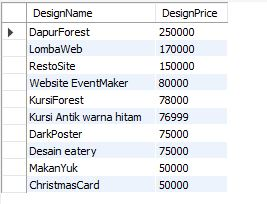
\includegraphics[width=0.4\textwidth]{view2}
			\caption{Hasil View 2}
		\end{figure}
	
	\item 	Melihat daftar transaksi dengan tipe pembayaran '\textit{ovo}' \\
			Source Code :
			\begin{lstlisting}[
				language=SQL,
				backgroundcolor=\color{backcolour},   
				commentstyle=\color{codegreen},
				keywordstyle=\color{magenta},
				numberstyle=\tiny\color{codegray},
				stringstyle=\color{codepurple},
				basicstyle=\ttfamily\footnotesize,
				breakatwhitespace=false,         
				breaklines=true,                 
				captionpos=b,                    
				keepspaces=true,                 
				numbers=left,                    
				numbersep=5pt,                  
	showspaces=false,                
	showstringspaces=false,
	showtabs=false,                  
	tabsize=2]
	create view design_harga_tertinggi as
	select B.DesignName, B.DesignPrice
	from DesignHeader A join DesignDetails B
	on A.DesignId = B.DesignId
	join User C
	on C.UserId = A.SupplierUserId
	order by B.DesignPrice desc;
	
	select * from design_harga_tertinggi;
	drop view design_harga_tertinggi;
			\end{lstlisting}
		Hasil:
		\\
		\begin{figure}[H]
			\centering
			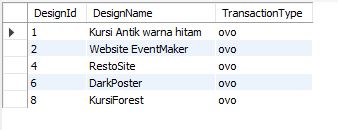
\includegraphics[width=0.6\textwidth]{view3}
			\caption{Hasil View 3}
		\end{figure}
	
	\item Melihat daftar data nama dan lokasi \textit{user} yang paling banyak melakukan transaksi
	Source Code :
	\begin{lstlisting}[
		language=SQL,
		backgroundcolor=\color{backcolour},   
		commentstyle=\color{codegreen},
		keywordstyle=\color{magenta},
		numberstyle=\tiny\color{codegray},
		stringstyle=\color{codepurple},
		basicstyle=\ttfamily\footnotesize,
		breakatwhitespace=false,         
		breaklines=true,                 
		captionpos=b,                    
		keepspaces=true,                 
		numbers=left,                    
		numbersep=5pt,                  
		showspaces=false,                
		showstringspaces=false,
		showtabs=false,                  
		tabsize=2]
		CREATE VIEW getMaxMin AS 
			SELECT
				UserInfo.Name,
				UserInfo.Location,
				count(*) as "Occurences"
			FROM
				UserInfo,
				User,
				UserInventory
			WHERE
				UserInfo.UserId = User.UserId AND
				User.UserId = UserInventory.Userid
			GROUP BY
				UserInventory.UserId
			ORDER BY
				count(*) DESC;
	\end{lstlisting}
	Hasil : 
	\\
	\begin{figure}[H]
		\centering
		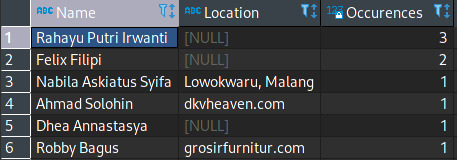
\includegraphics[width=0.4\textwidth]{view4}
		\caption{Hasil View 4}
	\end{figure}
\end{enumerate}
\subsubsection{User Triggers}
\begin{enumerate}
	\item	Fungsi \textit{trigger} untuk saat eksekusi \textit{insert}, melakukan \textit{insert} pada tabel 'UserPhoto' \\
			Source Code:
			\begin{lstlisting}[
				language=SQL,
				backgroundcolor=\color{backcolour},   
				commentstyle=\color{codegreen},
				keywordstyle=\color{magenta},
				numberstyle=\tiny\color{codegray},
				stringstyle=\color{codepurple},
				basicstyle=\ttfamily\footnotesize,
				breakatwhitespace=false,         
				breaklines=true,                 
				captionpos=b,                    
				keepspaces=true,                 
				numbers=left,                    
				numbersep=5pt,                  
				showspaces=false,                
				showstringspaces=false,
				showtabs=false,                  
				tabsize=2]
	Delimiter $$
	Create Trigger trig1
	after insert on User for each row 
	begin
	insert into UserPhoto value (NULL,new.UserId,'default.jpg');
	end $$
	Delimiter ;
	
	drop trigger trig1;
	insert into User value(NULL,'wasd@gmail.com','asd3',now(),1,0,0);
	select *from userphoto;
			\end{lstlisting}
		Hasil (Sebelum Trigger):
		\\
		\begin{figure}[H]
			\centering
			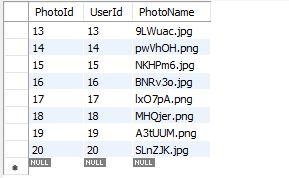
\includegraphics[width=0.6\textwidth]{trig1_before}
			\caption{Hasil Tabel Sebelum Trigger 1}
		\end{figure}
		Hasil (Setelah Trigger):
		\begin{figure}[H]
			\centering
			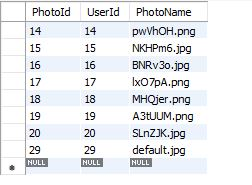
\includegraphics[width=0.6\textwidth]{trig1_after}
			\caption{Hasil Tabel Setelah Trigger 1}
		\end{figure}
	
	\item 	Fungsi \textit{trigger} untuk saat eksekusi \textit{delete}, memindahkan \textit{row} yang didelete menuju tabel \textit{temporary} \\
			Source Code:
			\begin{lstlisting}[
				language=SQL,
				backgroundcolor=\color{backcolour},   
				commentstyle=\color{codegreen},
				keywordstyle=\color{magenta},
				numberstyle=\tiny\color{codegray},
				stringstyle=\color{codepurple},
				basicstyle=\ttfamily\footnotesize,
				breakatwhitespace=false,         
				breaklines=true,                 
				captionpos=b,                    
				keepspaces=true,                 
				numbers=left,                    
				numbersep=5pt,                  
				showspaces=false,                
				showstringspaces=false,
				showtabs=false,                  
				tabsize=2]
	Delimiter $$
	Create Trigger trig2
	after delete on UserInfo for each row 
	begin
	create temporary table temp1(
	UserId INT(10) NOT NULL,
	Name VARCHAR(50) NOT NULL,
	Description TEXT,
	Company VARCHAR(48),
	Location VARCHAR(48),
	Website VARCHAR(48),
	PhoneNumber VARCHAR(16)
	);
	insert into temp1 values (old.UserId,old.name,old.description,old.company,old.location
	,old.website,old.phonenumber);
	end $$
	Delimiter ;
	
	delete from userInfo where userId=1;
			\end{lstlisting}
		Hasil (Sebelum Trigger):
		\\
		\begin{figure}[H]
			\centering
			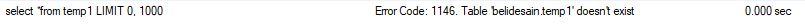
\includegraphics[width=\textwidth]{trig2_before}
			\caption{Hasil Tabel Sebelum Trigger 2}
		\end{figure}
		Hasil (Setelah Trigger):
		\begin{figure}[H]
			\centering
			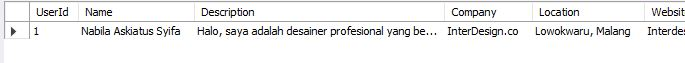
\includegraphics[width=\textwidth]{trig2_after}
			\caption{Hasil Tabel Setelah Trigger 2}
		\end{figure}
	
	\item	Fungsi \textit{trigger} untuk saat eksekusi \textit{insert}, memasukkan data kosong pada 'UserInfo' \\
			Source Code:
			\begin{lstlisting}[
				language=SQL,
				backgroundcolor=\color{backcolour},   
				commentstyle=\color{codegreen},
				keywordstyle=\color{magenta},
				numberstyle=\tiny\color{codegray},
				stringstyle=\color{codepurple},
				basicstyle=\ttfamily\footnotesize,
				breakatwhitespace=false,         
				breaklines=true,                 
				captionpos=b,                    
				keepspaces=true,                 
				numbers=left,                    
				numbersep=5pt,                  
				showspaces=false,                
				showstringspaces=false,
				showtabs=false,                  
				tabsize=2]
	Delimiter $$
	Create Trigger trig3
	after insert on User for each row 
	begin
	INSERT INTO UserInfo VALUES (new.UserId, NULL, NULL, NULL, NULL, NULL, NULL);
	end $$
	Delimiter ;
	
	insert into DesignFile value(NULL,'2','Naskle123','.svg');
			\end{lstlisting}
		Hasil (Sebelum Trigger):
		\\
		\begin{figure}[H]
			\centering
			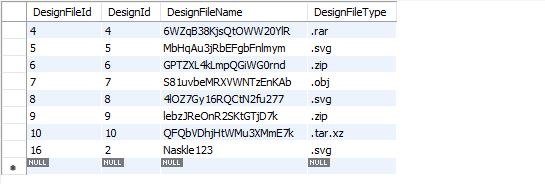
\includegraphics[width=\textwidth]{trig3_before}
			\caption{Hasil Tabel Sebelum Trigger 3}
		\end{figure}
		Hasil (Setelah Trigger):
		\begin{figure}[H]
			\centering
			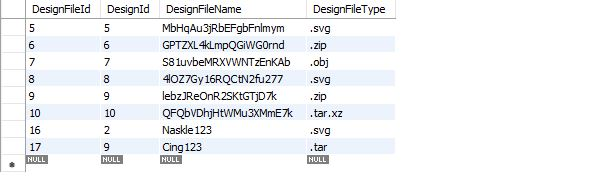
\includegraphics[width=\textwidth]{trig3_after}
			\caption{Hasil Tabel Setelah Trigger 3}
		\end{figure}
\end{enumerate}
\subsubsection{User Procedures}
\begin{enumerate}
	\item 	Fungsi \textit{Procedure} untuk melihat rata - rata \textit{rating} designer \\
	Source Code :
	\begin{lstlisting}[
		language=SQL,
		backgroundcolor=\color{backcolour},   
		commentstyle=\color{codegreen},
		keywordstyle=\color{magenta},
		numberstyle=\tiny\color{codegray},
		stringstyle=\color{codepurple},
		basicstyle=\ttfamily\footnotesize,
		breakatwhitespace=false,         
		breaklines=true,                 
		captionpos=b,                    
		keepspaces=true,                 
		numbers=left,                    
		numbersep=5pt,                  
		showspaces=false,                
		showstringspaces=false,
		showtabs=false,                  
		tabsize=2]
		Delimiter $$
		CREATE PROCEDURE getDesignerRating (
			IN DesignerId_param INT(10)
		)
		BEGIN
			SELECT 
				DesignerRating.DesignerId, 
				UserInfo.Name,
				AVG(DesignerRating.Rating) as Average
			FROM 
				DesignerRating, 
				UserInfo,User
			WHERE
				DesignerRating.DesignerId = User.UserId AND
				DesignerRating.DesignerId = DesignerId_param;
			END $$
		delimiter ;
		
		call getdesignerrating (20);
	\end{lstlisting} 
	Hasil : 
	\\
	\begin{figure}[H]
		\centering
		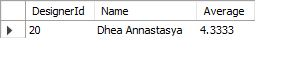
\includegraphics[width=0.4\textwidth]{proc1}
		\caption{Hasil Procedure 1}
	\end{figure}
	\item	Fungsi \textit{procedure} untuk melihat total \textit{like} pada desain \\
	Source Code :
	\begin{lstlisting}[
		language=SQL,
		backgroundcolor=\color{backcolour},   
		commentstyle=\color{codegreen},
		keywordstyle=\color{magenta},
		numberstyle=\tiny\color{codegray},
		stringstyle=\color{codepurple},
		basicstyle=\ttfamily\footnotesize,
		breakatwhitespace=false,         
		breaklines=true,                 
		captionpos=b,                    
		keepspaces=true,                 
		numbers=left,                    
		numbersep=5pt,                  
		showspaces=false,                
		showstringspaces=false,
		showtabs=false,                  
		tabsize=2]
		Delimiter $$
		CREATE PROCEDURE like_unlike(
			IN designId_param INT(10)
		)
		BEGIN
			SELECT
				DesignDetails.DesignName, 
				Count(DesignLikeCount.Likes) as 'Like'		
			FROM
				DesignHeader,
				DesignLikeCount,
				DesignDetails
			WHERE 
				DesignHeader.DesignId = DesignLikeCount.DesignId AND 
				DesignHeader.DesignId = DesignDetails.DesignId AND 
				DesignHeader.DesignId = designId_param and
				DesignLikeCount.Likes = 1;
		END $$
		delimiter ;
		
		call like_unlike (1);
	\end{lstlisting}
	Hasil : 
	\\
	\begin{figure}[H]
		\centering
		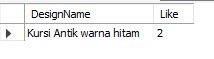
\includegraphics[width=0.4\textwidth]{proc2}
		\caption{Hasil Procedure 2}
	\end{figure}
	
	\item 	Fungsi \textit{procedure} untuk melihat total harga suatu \textit{event} \\
	Source Code:
	\begin{lstlisting}[
		language=SQL,
		backgroundcolor=\color{backcolour},   
		commentstyle=\color{codegreen},
		keywordstyle=\color{magenta},
		numberstyle=\tiny\color{codegray},
		stringstyle=\color{codepurple},
		basicstyle=\ttfamily\footnotesize,
		breakatwhitespace=false,         
		breaklines=true,                 
		captionpos=b,                    
		keepspaces=true,                 
		numbers=left,                    
		numbersep=5pt,                  
		showspaces=false,                
		showstringspaces=false,
		showtabs=false,                  
		tabsize=2]
		DELIMITER $$
		CREATE PROCEDURE total_ticket(
			IN ExpoTransactionId_param INT(10)
		)
		BEGIN
			SELECT
				ExpoEventDetails.ExpoEventTitle,
				ExpoEventDetails.TicketPrice,
				ExpoTransactionHeader.TicketQty,
				(ExpoEventDetails.TicketPrice * ExpoTransactionHeader.TicketQty) as "Total"
			FROM 
				ExpoTransactionHeader,
				ExpoEvent,
				ExpoEventDetails
			WHERE
				ExpoTransactionHeader.ExpoEventId = ExpoEvent.ExpoEventId AND
				ExpoEvent.ExpoEventId = ExpoEventDetails.ExpoEventId AND
				ExpoEvent.ExpoEventId = ExpoTransactionid_param;
			END $$
		DELIMITER ;
	\end{lstlisting}
	Hasil:
	\\
	\begin{figure}[H]
		\centering
		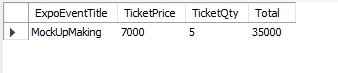
\includegraphics[width=0.6\textwidth]{proc3}
		\caption{Hasil Procedure 3}
	\end{figure}

	\item 	Fungsi \textit{procedure} untuk menghitung \textit{max}, \textit{min}, dan total tiket dari sebuah \textit{event} \\
	Source Code:
	\begin{lstlisting}[
		language=SQL,
		backgroundcolor=\color{backcolour},   
		commentstyle=\color{codegreen},
		keywordstyle=\color{magenta},
		numberstyle=\tiny\color{codegray},
		stringstyle=\color{codepurple},
		basicstyle=\ttfamily\footnotesize,
		breakatwhitespace=false,         
		breaklines=true,                 
		captionpos=b,                    
		keepspaces=true,                 
		numbers=left,                    
		numbersep=5pt,                  
		showspaces=false,                
		showstringspaces=false,
		showtabs=false,                  
		tabsize=2]
		Delimiter $$
		CREATE procedure procedure1 (in sort_parameter varchar(4))
		begin
		if sort_parameter='DESC' then
		select expoevent.expoeventid, ExpoEventDetails.ExpoEventTitle, ticketqty*ticketprice
		as Total_Penjualan_Ticket from ExpoEventDetails,ExpoEvent,ExpoTransactionHeader
		where ExpoEventDetails.ExpoEventId=ExpoEvent.ExpoEventId 
		and ExpoEvent.ExpoEventId=ExpoTransactionHeader.ExpoEventId and ExpoTransactionHeader.IsSuccess=1 
		order by Total_Penjualan_Ticket desc;
		
		elseif sort_parameter='ASC' then
		select expoevent.expoeventid, ExpoEventDetails.ExpoEventTitle, ticketqty*ticketprice
		as Total_Penjualan_Ticket from ExpoEventDetails,ExpoEvent,ExpoTransactionHeader
		where ExpoEventDetails.ExpoEventId=ExpoEvent.ExpoEventId 
		and ExpoEvent.ExpoEventId=ExpoTransactionHeader.ExpoEventId and ExpoTransactionHeader.IsSuccess=1 
		order by Total_Penjualan_Ticket asc;
		end if;
		end $$
		delimiter ;
	\end{lstlisting}
	Hasil:
	\\
	\begin{figure}[H]
		\centering
		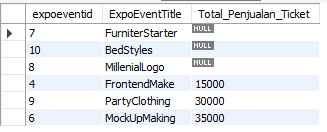
\includegraphics[width=0.6\textwidth]{proc4_asc}
		\caption{Hasil Procedure 4 (ascending)}
	\end{figure}
	\begin{figure}[H]
		\centering
		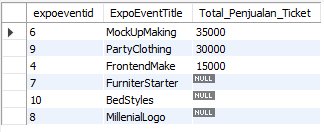
\includegraphics[width=0.6\textwidth]{proc4_desc}
		\caption{Hasil Procedure 4 (descending)}
	\end{figure}

	\item 	Fungsi \textit{procedure} untuk melihat desain dan nama desainer paling favorit di setiap kategori desain \\
	Source Code:
	\begin{lstlisting}[
		language=SQL,
		backgroundcolor=\color{backcolour},   
		commentstyle=\color{codegreen},
		keywordstyle=\color{magenta},
		numberstyle=\tiny\color{codegray},
		stringstyle=\color{codepurple},
		basicstyle=\ttfamily\footnotesize,
		breakatwhitespace=false,         
		breaklines=true,                 
		captionpos=b,                    
		keepspaces=true,                 
		numbers=left,                    
		numbersep=5pt,                  
		showspaces=false,                
		showstringspaces=false,
		showtabs=false,                  
		tabsize=2]
		CREATE PROCEDURE Desain_Favorit ()
		select
		DesignName1,
		CategoryName,
		DesainerName
		from
		(select
		UserInfo.UserId as UserId,
		DesignDetails.DesignName as DesignName1,
		count(*) as DesignCount,
		DesignCategories.CategoryName as CategoryName,
		UserInfo.Name as DesainerName
		from 
		DesignTransactionHeader,
		User,
		UserInfo,
		DesignHeader,
		DesignDetails,
		DesignCategories
		where
		User.UserId = UserInfo.UserId and
		User.UserId = DesignTransactionHeader.BuyerUserId and 
		DesignTransactionHeader.DesignId = DesignHeader.DesignId and
		DesignHeader.DesignId = DesignDetails.DesignId and
		DesignCategories.CategoryId = DesignHeader.CategoryId
		group by
		DesignDetails.DesignName) a,
		DesignDetails
		where
		DesignName1 = DesignDetails.DesignName
		group by 
		CategoryName;
		
		CALL Desain_Favorit;
	\end{lstlisting}
	Hasil:
	\\
	\begin{figure}[H]
		\centering
		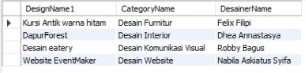
\includegraphics[width=0.6\textwidth]{proc5}
		\caption{Hasil Procedure 5}
	\end{figure}

	\item 	Fungsi \textit{procedure} untuk melihat tanggal dengan \textit{profit} penjualan maksimal dan minimal \\
	Source Code:
	\begin{lstlisting}[
		language=SQL,
		backgroundcolor=\color{backcolour},   
		commentstyle=\color{codegreen},
		keywordstyle=\color{magenta},
		numberstyle=\tiny\color{codegray},
		stringstyle=\color{codepurple},
		basicstyle=\ttfamily\footnotesize,
		breakatwhitespace=false,         
		breaklines=true,                 
		captionpos=b,                    
		keepspaces=true,                 
		numbers=left,                    
		numbersep=5pt,                  
		showspaces=false,                
		showstringspaces=false,
		showtabs=false,                  
		tabsize=2]
		Delimiter $$
		create procedure proc4(in min_max char(3))
		begin create temporary table temp1(penjualan int(50),tanggal datetime);
		
		insert into temp1
		select sum(designdetails.designprice) as penjualan,designtransactiondetails.transactiondate
		from designtransactiondetails,designdetails,designtransactionheader,designheader
		where designtransactiondetails.designtransactionid=designtransactionheader.designtransactionid
		and designdetails.designid=designheader.designid and 
		designheader.designid=designtransactionheader.designtransactionid and
		designtransactionheader.issuccess=1 group by cast(transactiondate as date)
		union all
		select designerinfo.designerprice as penjualan,designertransactiondetail.assigneddate
		from designertransactiondetail,user,designertransactionheader,designerinfo
		where designertransactiondetail.designertransactionid=designertransactionheader.designertransactionid
		and designertransactionheader.designerid=user.userid and
		user.userid=designerinfo.designerid and
		designertransactionheader.issuccess=1 and designertransactiondetail.confirmed=1 
		group by cast(assigneddate as date)
		union all
		select expotransactionheader.ticketqty* #kali
		expoeventdetails.ticketprice as penjualan,
		expotransactiondetails.expotransactiondate
		from expotransactiondetails,Expotransactionheader,expoevent,expoeventdetails
		where expotransactiondetails.expotransactionid=expotransactionheader.Expotransactionid
		and expotransactionheader.expoeventid=expoevent.expoeventid and
		expoevent.expoeventid=expoeventdetails.expoeventid and
		expotransactionheader.issuccess=1 group by cast(expotransactiondate as date);
		
		if min_max='min' then
		select cast(tanggal as date) as tanggalmax, max(a.total) as maksimal_penjualan
		from (select cast(tanggal as date) as tanggal_penjualan, sum(penjualan) as total 
		from temp1 group by tanggal_penjualan) a, temp1 where cast(tanggal as date) = tanggal_penjualan
		group by cast(tanggal as date) order by maksimal_penjualan asc limit 1;
		elseif min_max='max' then select cast(tanggal as date) as tanggalmax, max(a.total) as maksimal_penjualan
		from(select cast(tanggal as date) as tanggal_penjualan, sum(penjualan) as total from temp1 group by
		tanggal_penjualan) a,temp1 where cast(tanggal as date) = tanggal_penjualan group by cast(tanggal as date)
		order by maksimal_penjualan desc limit 1;
		end if;
		end $$
		Delimiter ;
	\end{lstlisting}
	Hasil:
	\\
	\begin{figure}[H]
		\centering
		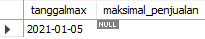
\includegraphics[width=0.6\textwidth]{proc6_max}
		\caption{Hasil Procedure 6 (\textit{min})}
	\end{figure}
	\begin{figure}[H]
	\centering
	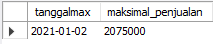
\includegraphics[width=0.6\textwidth]{proc6_min}
	\caption{Hasil Procedure 6 (\textit{max})}
\end{figure}
\end{enumerate}